\documentclass[12pt,onecolumn,draftcls]{IEEEtran}
\usepackage{amsmath,amssymb,amsfonts,bm}
\usepackage{color}
\usepackage{pgf}
\usepackage{tikz,pgf}
\tikzset{font={\fontsize{10pt}{12}\selectfont}}

\begin{document}

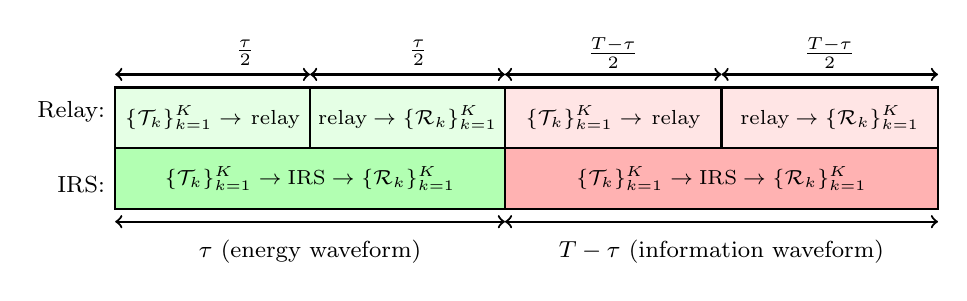
\begin{tikzpicture}[scale=1.1,every node/.style={scale=1.05}]
 \draw[<->,thick] (-.5,.85)--++(2.25,0);
 \node [left] at (-.5,.425) {\footnotesize Relay:};
\node [left] at (-.5,-.425) {\footnotesize IRS:};
 \draw[<->,thick] (-.5,-.85)--++(4.5,0);
 \draw[<->,thick] (1.75,.85)--++(2.25,0);
 \draw[<->,thick] (4,.85)--++(2.5,0);
 \draw[<->,thick] (4,-.85)--++(5,0);
 \draw[<->,thick] (6.5,.85)--++(2.5,0);
 \draw[thick,fill=green!30] (-.5,-.7) rectangle ++(4.5,.7) node[midway]{\scriptsize $\{\mathcal{T}_k\}_{k=1}^K\rightarrow\hspace{2pt}$IRS$\hspace{2pt}\rightarrow \{\mathcal{R}_k\}_{k=1}^K$} ;
 \draw[thick,fill=green!10] (-.5,0) rectangle ++(2.25,.7) node[midway]{\scriptsize $\{\mathcal{T}_k\}_{k=1}^K \rightarrow$\hspace{3pt}relay};
 \draw[thick,fill=green!10] (1.75,0) rectangle ++(2.25,.7) node[midway]{\scriptsize relay\hspace{2pt}$\rightarrow\{\mathcal{R}_k\}_{k=1}^K$} ;
 \draw[thick,fill=red!30] (4,-.7) rectangle ++(5,.7) node[midway]{\scriptsize $\{\mathcal{T}_k\}_{k=1}^K \rightarrow\hspace{2pt}$IRS$\hspace{2pt}\rightarrow \{\mathcal{R}_k\}_{k=1}^K$} ;
 \draw[thick,fill=red!10] (4,0) rectangle ++(2.5,.7) node[midway]{\scriptsize $\{\mathcal{T}_k\}_{k=1}^K \rightarrow$\hspace{3pt}relay};
 \draw[thick,fill=red!10] (6.5,0) rectangle ++(2.5,.7) node[midway]{\scriptsize relay$\hspace{2pt}\rightarrow \{\mathcal{R}_k\}_{k=1}^K$};
 \node [] at (1,1.1) {\footnotesize $\frac{\tau}{2}$};
 \node [] at (1.75,-1.2) {\footnotesize $\tau$ (energy waveform)};
 \node [] at (3,1.1) {\footnotesize $\frac{\tau}{2}$};
 \node [] at (5.25,1.1) {\footnotesize $\frac{T-\tau}{2}$};
 \node [] at (6.5,-1.2) {\footnotesize $T- \tau$ (information waveform)};
 \node [] at (7.75,1.1) {\footnotesize $\frac{T-\tau}{2}$};
 \end{tikzpicture}

\end{document}